\section{Conic and Invariant Detection}

\subsection{Curve Type}

As shown in \cref{fig:09-conic-invariants}, when one or more loci are displayed, the app  indicates in the lower right-hand side of the corresponding control group, the curve type of the locus (detected via least-squares curve fitting). The following codes are used:

\begin{itemize}
    \item \texttt{X}: non-conic
    \item \texttt{E}: ellipse
    \item \texttt{H}: hyperbola
    \item \texttt{P}: parabola (very rare)
    \item \texttt{L}: line or segment
    \item \texttt{*}: a stationary point.
\end{itemize}

The same code is also appended (in parenthesis) to the (moving) triangle center being displayed, for example, \cref{fig:09-conic-invariants}, \texttt{X2(E),X3(E),X4(E)}, indicate the loci of barycenter, circumcenter, and orthocenter are ellipses over billiard 3-periodics.

\begin{figure}
    \centering
    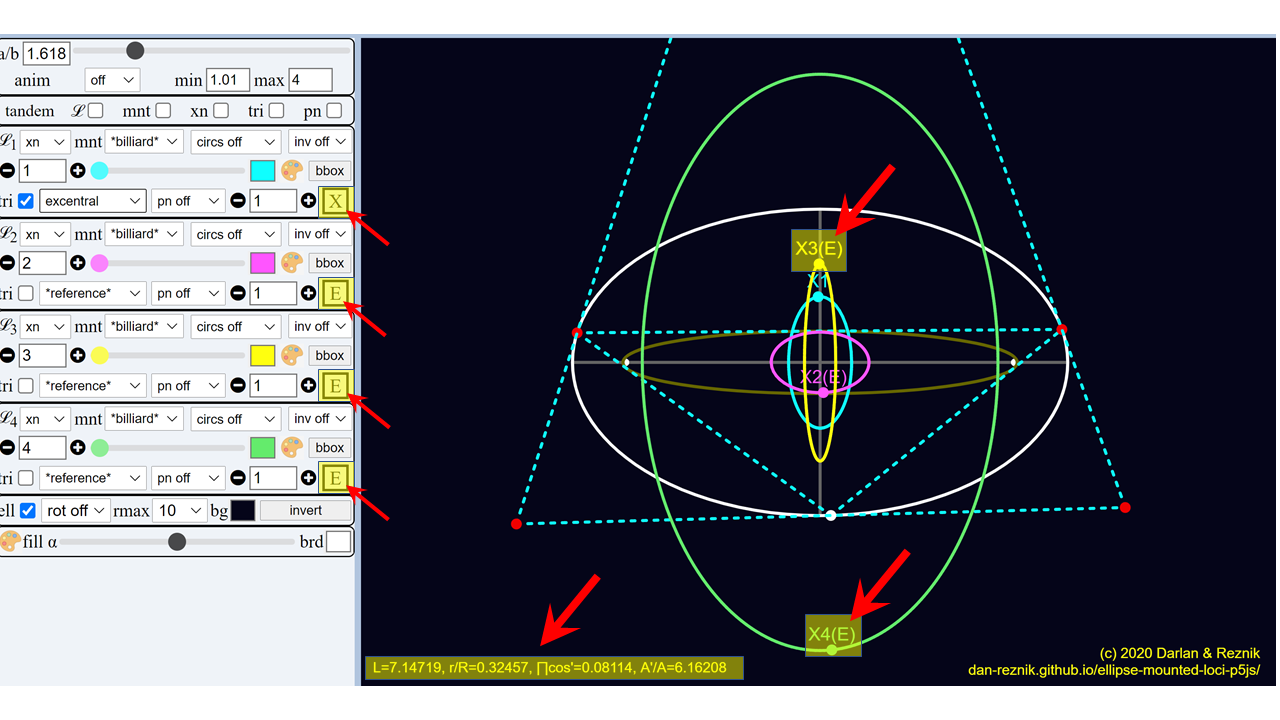
\includegraphics[width=.8\textwidth]{pics_09_120_conic_invariants.png}
    \caption{An indication as to curve type of each locus appears in a small box in the lower right-hand side of each control group. In the picture, \texttt{X} means the first locus (incenter over the excentral family) is non-conic. An \texttt{E} in the remainder 3 channels indicates their loci are ellipses. Notice the same indicator is appended to the instantenous location of the triangle centers being tracked, e.g., \texttt{X3(E)} indicates the locus of the circumcenter is an ellipse. \href{https://bit.ly/3uXndpa}{Live}}
    \label{fig:09-conic-invariants}
\end{figure}

\subsection{Detection of Metric Invariants}

The app also reports when certain basic, metric quantities are invariant, currently over triangles in the first channel only. These appear as a single line at the bottom of the animation area of a given experiment, see \cref{fig:09-conic-invariants}. In the example, the following line of text is reported:

\[ L=7.14..., r/R=0.32..., \prod\cos'=0.0811, A'/A=6.6... \]

In turn, this means that perimeter $L$ and ratio $r/R$ of inradius-to-circumradius are  numerically invariant over the reference family selected in channel 1, and that the product $\prod\cos'$ of cosines, and ratio $A'/A$ of derived-by-reference areas is constant (these are observations first introduced in \cite{reznik2020-intelligencer}).

Reported invariants appear unprimed to refer to the reference triangle in a given family. Primed quantities will appear when a derived triangle has been selected (e.g., ``excentral''), allowing for mutual comparison. 

The following quantities are currently reported, when numerically invariant:

\begin{itemize}
    \item $L,A$: perimeter and area
    \item $r,R$: inradius and circumradius
    \item $r/R$: ratio of inradius-to-circumradius, tantamount to invariant sum of cosines since $\sum{\cos}=1+r/R$.
    \item $\cot(\omega)$: the cotangent of the Brocard angle
    \item $\sum{s^2},\sum{1/s},\sum{s^{-2}}$: sum of squared, reciprocal, or reciprocal-squared sidelengths, respectively.
    \item $\prod\cos$: the product of internal
    \item $\prod{s}$: the product of sidelengths
    \item $R_c$: if a circle is selected via the circle menu (\cref{sec:09-inversion-circles}), whether its radius is constant.
\end{itemize}

Also reported whenever a derived triangle is selected, are one of $L'/L$, $A'/A$, $A'.A$, $R_c'/R_c$ if these are invariant.